\documentclass[dvipdfmx]{jsarticle}
\usepackage[dvipdfmx]{graphicx}
\usepackage{amsmath, amssymb}
\usepackage{mathtools}
\usepackage{here}
\begin{document}
\title{週間進捗報告}
\author{権藤陸}
\maketitle
\section{今週の進捗}
\begin{itemize}
    \item Person Reidentification Based on Automotive Radar Point Cloudsの読み込み
    \item 他4文献の確認
\end{itemize}
\section{レーダの原理}
本研究で用いられたレーダは,FMCW(周波数変調連続波)と呼ばれるミリ波を用いたレーダである.距離,方向,速度を測定する目的で,周波数変調された信号を連続的に送信する.
\begin{itemize}
    \item 距離測定

下図のように周波数が直線的に変化するチャープ信号を送受信することで距離測定が可能である.

    \begin{figure}[H]
    \begin{center}
    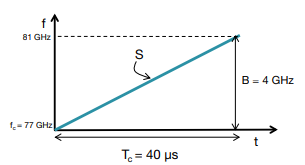
\includegraphics[width=0.75\linewidth]{./img/charp_signal.png}
    \end{center}
    \caption{チャープ信号}
    \end{figure}

    \item 速度測定

    ある一定時間で分離された2つのチャープ信号を送り,反射してきたチャープをFFTで処理し,その位相差から速度を測定する.

    \item 方角測定

    測定対象の物体と各アンテナとの距離には差があり,FFTのピークに位相差が生じる.この位相の変化を利用して角度を推定する.
\end{itemize}

\section{関連研究}
\begin{itemize}
    \item カメラベースの容姿に依存するReIDシステム
    \item レーダベースの歩行特徴を抽出するReID
    \item LiDAR・深度カメラによる点群の深層学習
\end{itemize}
\section{提案法}
\begin{figure}[htbp]
\begin{center}
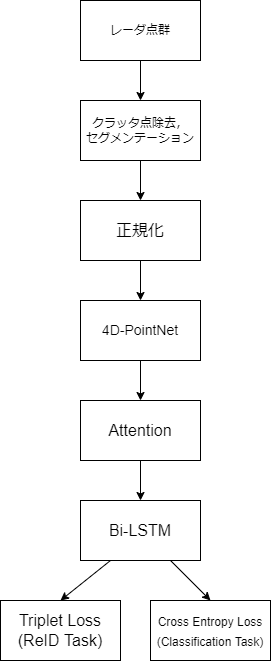
\includegraphics[width=0.25\linewidth]{./img/ReID_Model.png}
\end{center}
\caption{提案法の処理の流れとモデル}
\end{figure}

\section{他4つの文献}
\begin{itemize}
    \item FMCWレーダを用いて,家の中を動く人間の歩行特徴を軽量のCNNで学習・分類\cite{home}
    \item FMCWレーダのデータセットからmicro-doppler signatureを抽出し,提案されたマルチスケールCNNで学習し,個人認証に利用\cite{multi}
    \item FMCWレーダのデータから抽出したドップラースペクトログラムにFFTをかけて得た歩調速度図に,GPN(Gaussian Prototypical Network)により分類\cite{gpn}
    \item FMCWレーダを用いる.歩行特徴量を提案されたトリプルジョイントロス(ソフトマックスロス+センターロス+コサインロス)で分類.\cite{loss}
    
いずれも再認識を行う研究ではない
\end{itemize}

\section{計画}
\begin{itemize}
    \item ReID論文の読み込み
    \item スライド作成
\end{itemize}

\begin{thebibliography}{}
\bibitem{home} Zhaoyang Xia, "Genming Ding, Hui Wang, and Feng Xu, Person Identification With Millimeter-Wave Radar in Realistic Smart Home Scenarios", \textit{IEEE GEOSCIENCE AND REMOTE SENSING LETTERS}, Vol. 19, 2022
\bibitem{multi} YuHuang, Enshuo Jiang, Haodong Xu, and Guangbo Zhang, "Person identification using a new CNN-based method and radar gait micro-Doppler signatures", \textit{Journal of Physics: Conference Series}, 2258 012044, 2022
\bibitem{gpn} Usman Niazi, Souvik Hazra, Avik Santra, Robert Weigel, "Radar-Based Efficient Gait Classification using Gaussian Prototypical Networks", \textit{IEEE Radar Conference}, 20844114, 2021
\bibitem{loss} 
Y. Yang, B. Huang and Z. Ni, "Open-set Person Identification with Triple-Joint Loss Based on Radar Gait Micro-Doppler Signatures," \textit{2022 7th International Conference on Intelligent Computing and Signal Processing (ICSP)}, 2022, pp. 1787-1791, doi: 10.1109/ICSP54964.2022.9778544.
\end{thebibliography}
\end{document}